%!TEX root = main.tex
Figure~\ref{fig:normalop}
\begin{figure}
  \centering
  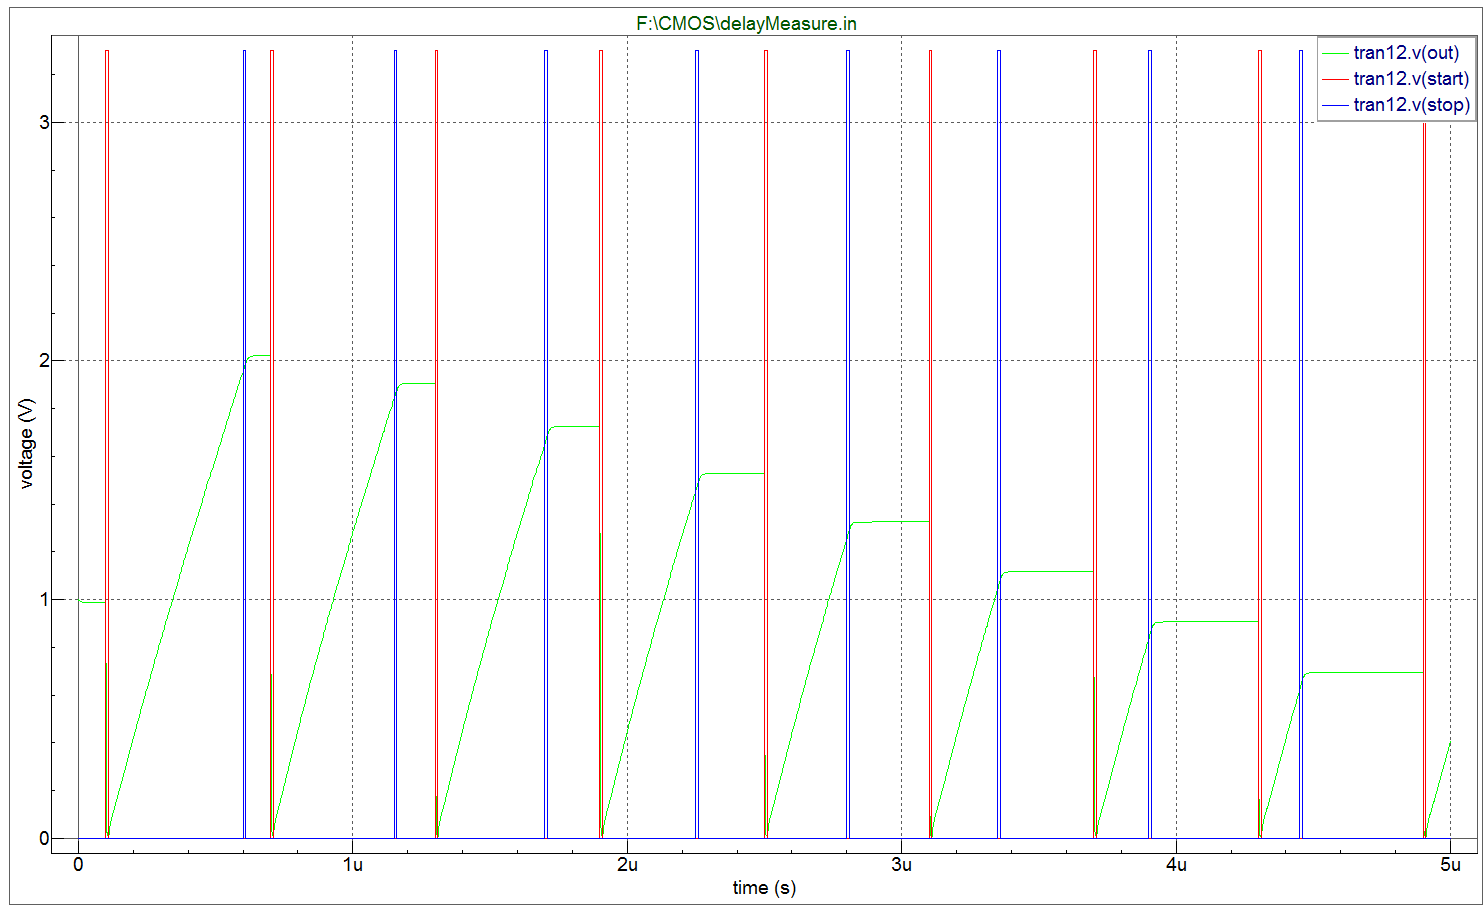
\includegraphics[width=\textwidth]{normalop.png}
  \caption{Delay measurement device under normal operation.\label{fig:normalop}}
\end{figure}
shows the device working in normal conditions and proves that it is working as it is supposed to.
In the next subsections, we will examine its properties more closely, starting with the most important one, its static characteristic.

\subsection{Static Characteristic}
Figure~\ref{fig:carac}
\begin{figure}
  \centering
  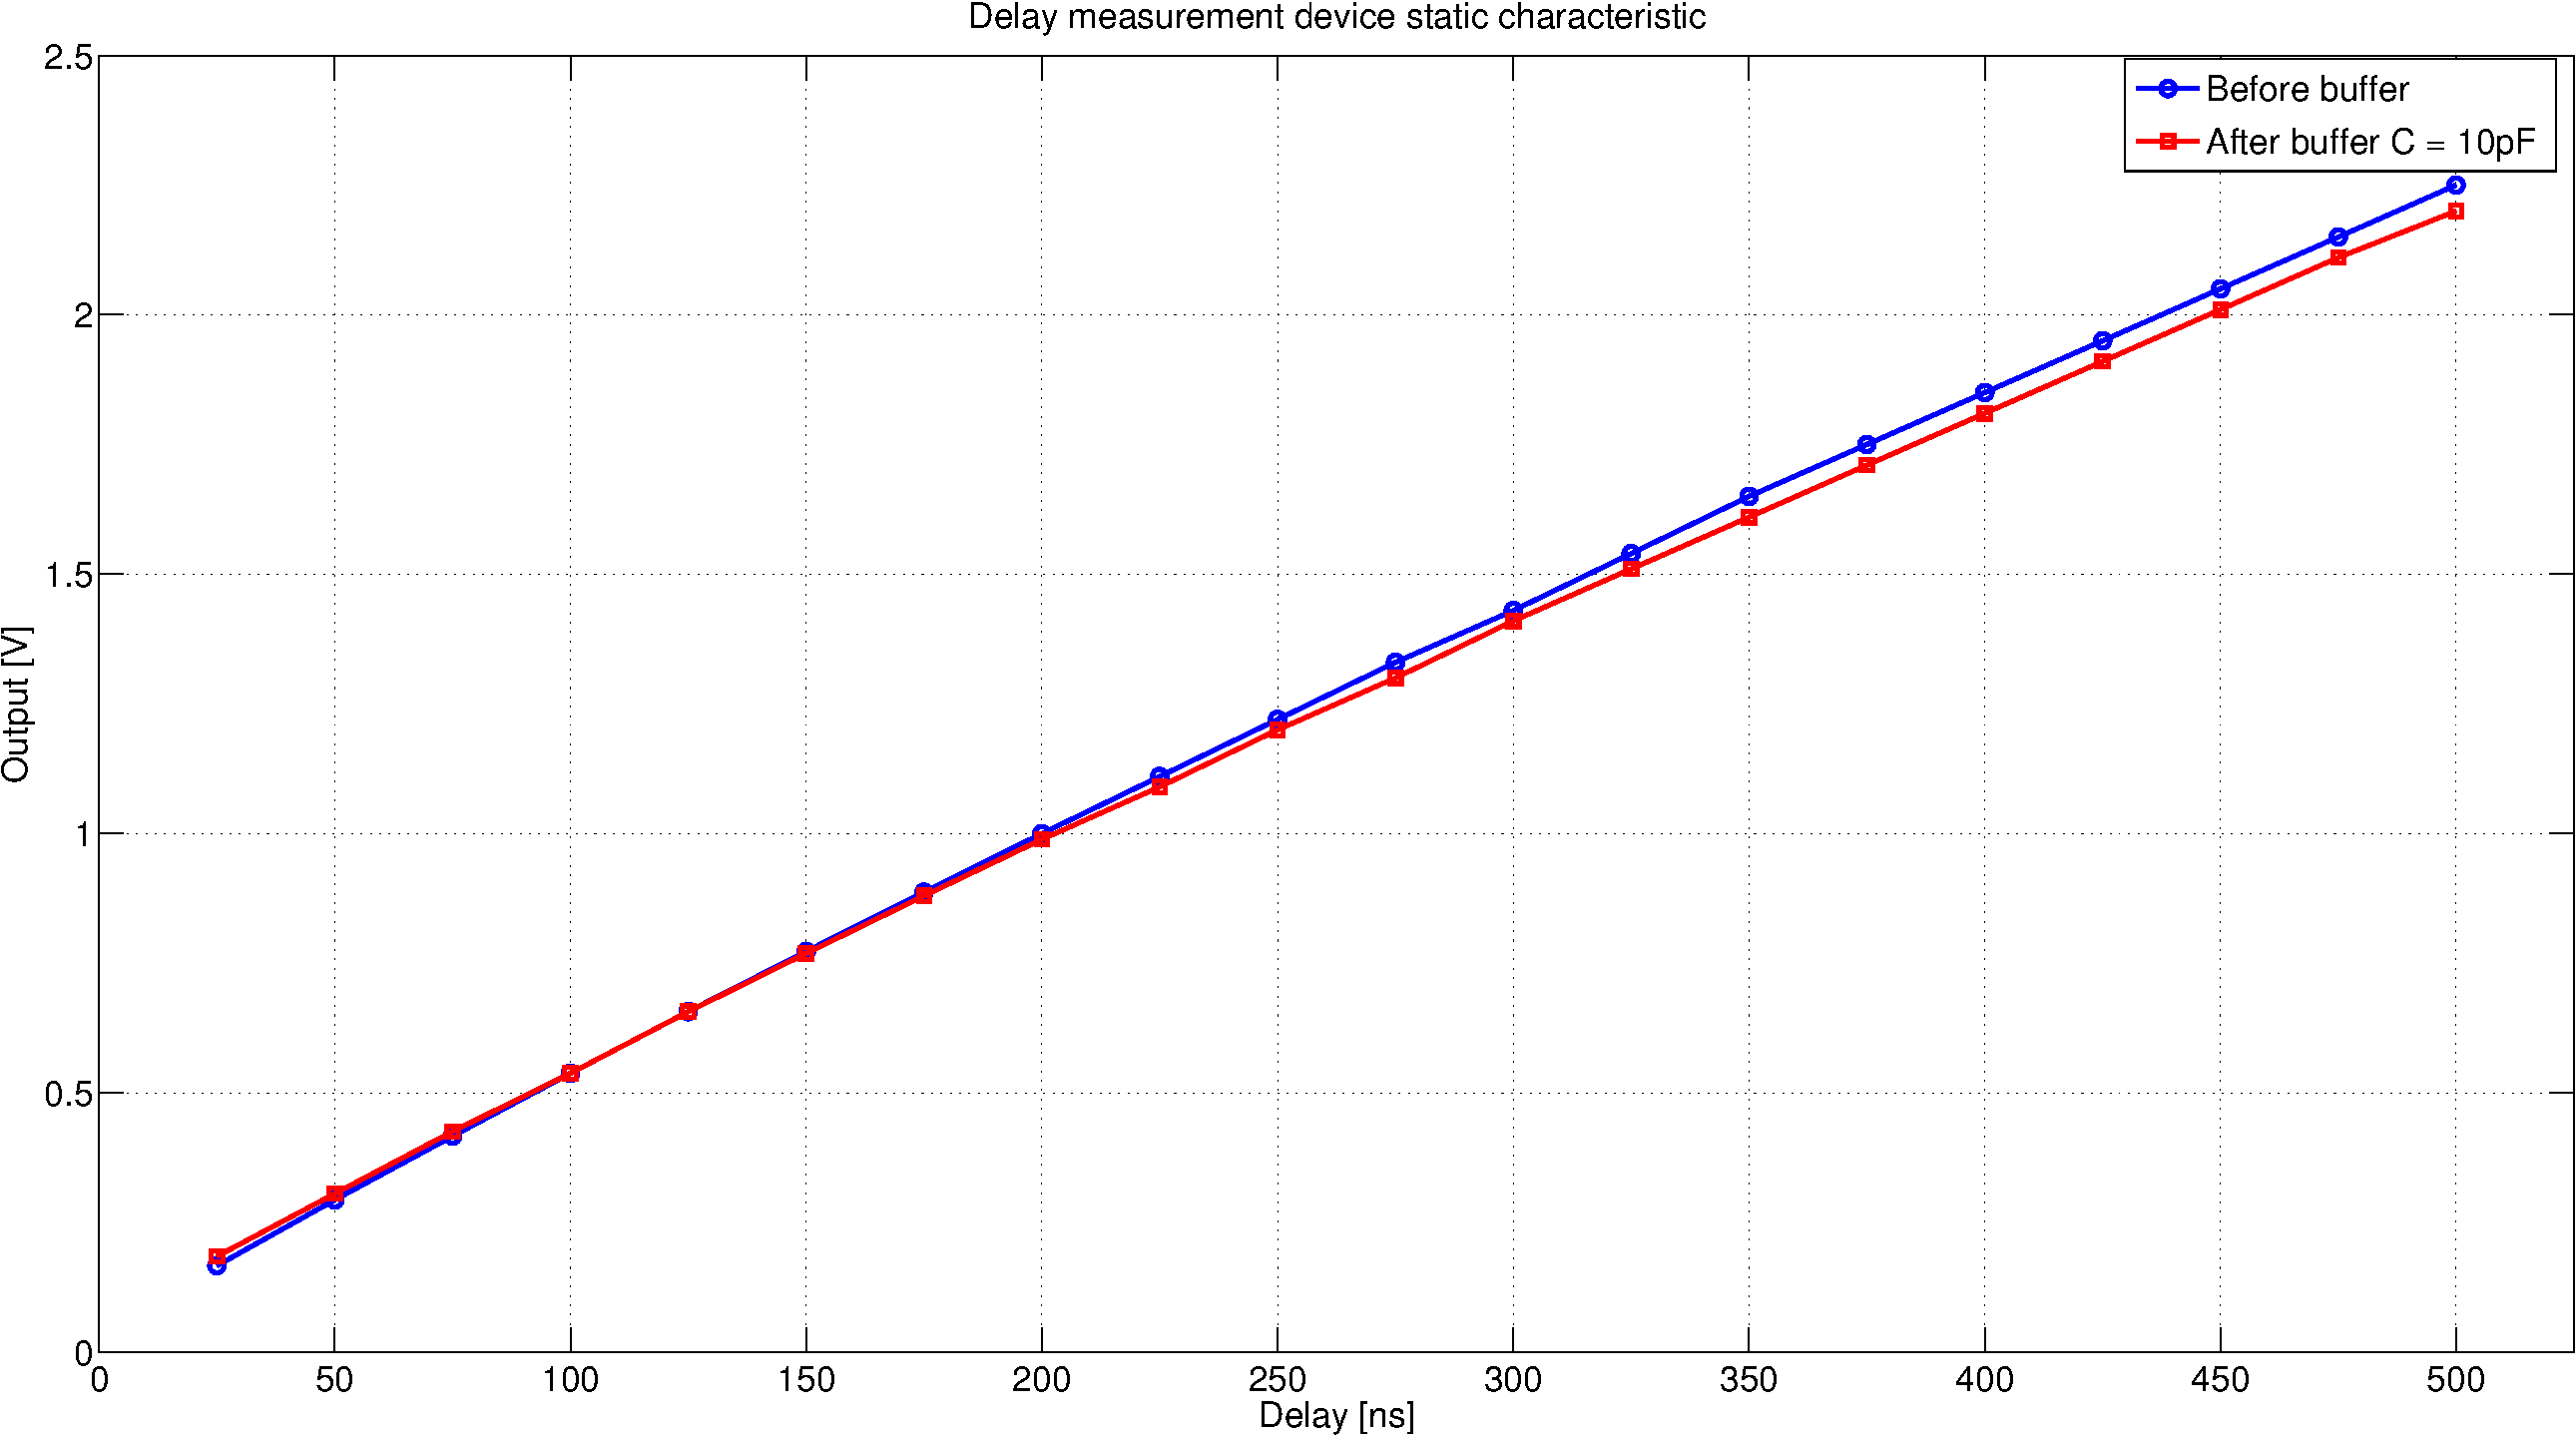
\includegraphics[width=\textwidth]{carac.pdf}
  \caption{Static characteristic of the device.\label{fig:carac}}
\end{figure}
shows the static characteristic of the device, before and after the output stage. The characteristic is pretty linear in both cases.
The output stage changes the slope a little because the static error changes slightly across the output range, but the linearity is preserved, which is the most important aspect.

\subsection{Output Range}
Figure~\ref{fig:carac} shows that the output ranges from \SI{118}{\milli\volt} for a \SI{10}{\nano\second} delay to \SI{2.20}{\volt} for a \SI{500}{\nano\second} delays.
Figure~\ref{fig:range}
\begin{figure}
  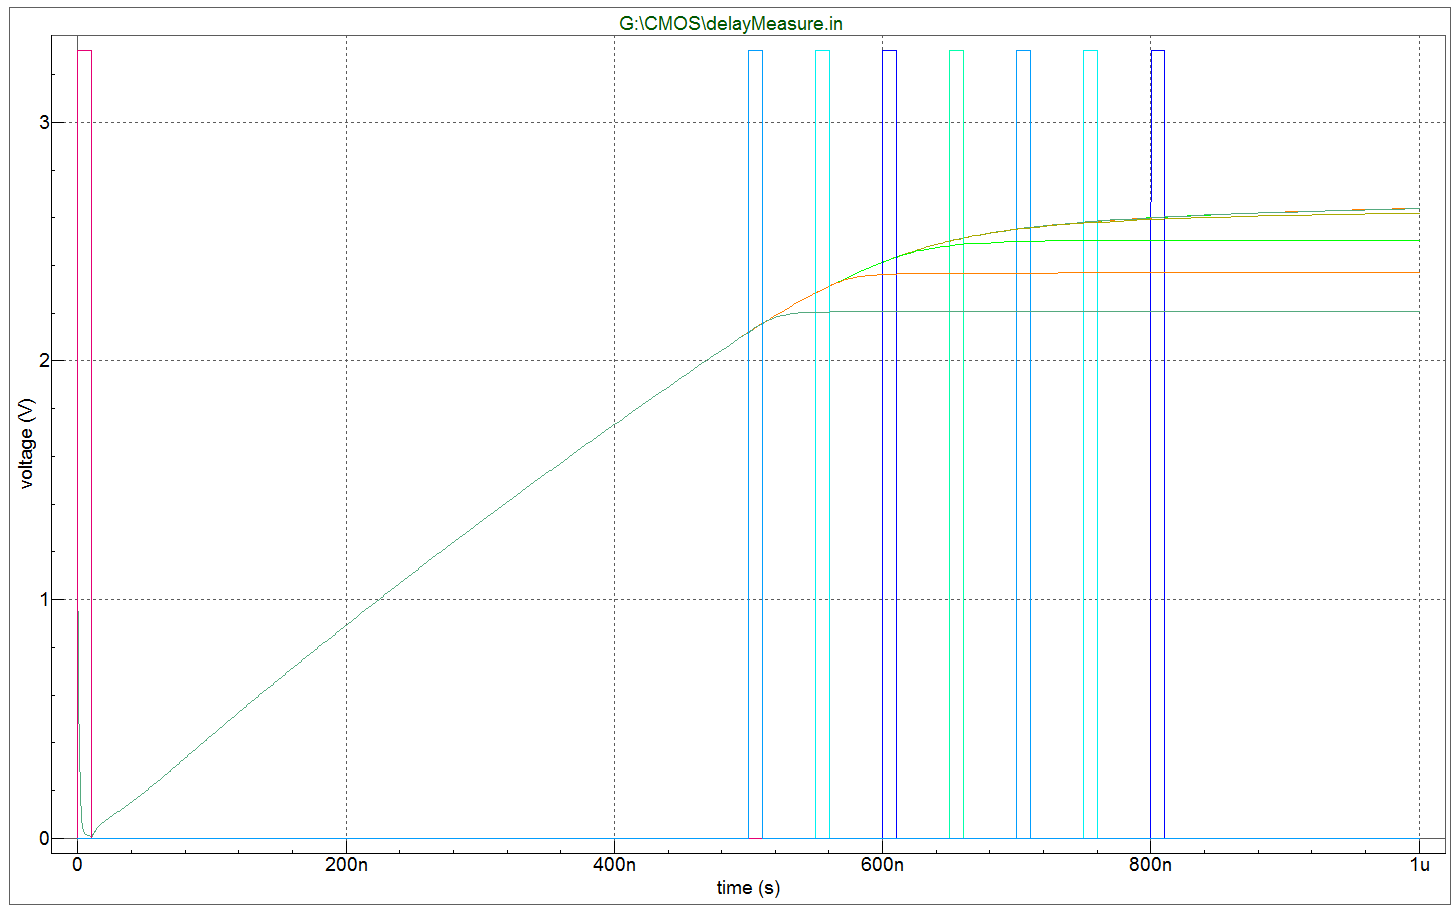
\includegraphics[width=\textwidth]{range.png}
  \caption[Output range limits of the device.]{Output range limits of the device. Shortest delay (dark green): \SI{500}{\nano\second} delay, other tested delays are in increments of \SI{50}{\nano\second}.\label{fig:range}}
\end{figure}
shows how the device behaves for longer delays.
The output stays linear for delays slightly outside of the nominal range, but then starts to lose linearity very quickly.
This means that the device is correctly sized from that point of view and that the near full output range is used during normal operation.

\subsection{Imperfections}
The device has two main sources of imperfections.
First, as presented in subsection \ref{sub:rampsize}, there is a capacitive coupling between the output of \blk{rampgen} and its digital input \sig{charge}, which means that there are small steps at the output of the device on falling edges of \sig{start} and \sig{stop}.

Secondly, the device is not perfectly memoryless.
This is because there is a capacitive path between the output of the device and \sig{vbias}, through the OTA.
This means that the very steep falling edge which happens on the output at every reset pulls \sig{vbias} down.
The effect on \sig{vbias} depends on the height of the edge and influences the current that charges the capacitor to provide \sig{measurement}.
A measurement is thus slightly influenced by the previous one: the device has some hysteresis.

To avoid this, the user can consider this effect as a transient, run multiple identical measurements back to back and only keep the last one so that the output doesn't depend on the unknown state of \sig{vbias} anymore.
